\documentclass[t]{beamer}
\usetheme{Copenhagen}
\setbeamertemplate{headline}{} % remove toc from headers
\beamertemplatenavigationsymbolsempty

\usepackage{amsmath, array, tikz, bm, pgfplots, tcolorbox, tkz-euclide}
\usetkzobj{all}
\pgfplotsset{compat = 1.16}

\title{Measuring Angles}
\author{}
\date{}

% \begin{tcolorbox}[colframe=green!20!black, colback = green!30!white,title=\textbf{TITLE}]

\AtBeginSection[]
{
  \begin{frame}
    \frametitle{Objectives}
    \tableofcontents[currentsection]
  \end{frame}
}

\begin{document}

\begin{frame} 
\maketitle
\end{frame}

\section{Find the area of irregular shapes}

\begin{frame}{Perimeter and Area}
\begin{tcolorbox}[colframe=green!20!black, colback = green!30!white,title=\textbf{Perimeter}]
The \textbf{perimeter} of a polygon is the sum of the lengths of its sides.
\end{tcolorbox}
\vspace{10pt} \pause

\begin{tcolorbox}[colframe=green!20!black, colback = green!30!white,title=\textbf{Area}]
The \textbf{area} of a polygon is the number of square units it uses (i.e. how much space it takes up on paper).
\end{tcolorbox}
\vspace{10pt}	\pause

We can find the areas and perimeters of irregular shapes by dividing it into simpler shapes and either adding or subtracting individual areas.
\end{frame}

\begin{frame}{Areas and Perimeters of Common Shapes}
\begin{tabular}{p{0.5\textwidth}p{0.4\textwidth}}
\textbf{Triangle}    	&   \textbf{Square}  \\[5pt]
$A = \frac{1}{2}bh$ 	&   $A = s^2$   		\\[10pt]
\begin{tikzpicture}
    \tkzDefPoints{0/0/A, 3/0/B, 1/2/C}
    \tkzDrawPolygon(A,B,C)
    \tkzLabelSegment[below](A,B){$b$}
    \tkzDefLine[orthogonal=through C](B,A) 
    \tkzGetPoint{D}
    \tkzInterLL(C,D)(A,B)
    \tkzGetPoint{E}
    \tkzDrawSegment[dashed](C,E)
    \tkzLabelSegment[below right](C,E){$h$}
\end{tikzpicture}
&   \raisebox{2.4cm}{
\begin{tikzpicture}
    \tkzDefPoints{2/2/A, 4/2/B, 4/4/C, 2/4/D}
    \tkzDrawPolygon(A,B,C,D)
    \tkzLabelSegments[below](A,B){$s$}
    \tkzLabelSegments[right](B,C){$s$}
    \tkzMarkRightAngle(C,B,A)
\end{tikzpicture}}
\end{tabular}
\end{frame}

\begin{frame}{Areas and Perimeters of Common Shapes}
\begin{tabular}{p{0.5\textwidth}p{0.4\textwidth}}
\textbf{Rectangle}   	&   \textbf{Circle}    					\\[5pt]
$A = lw$    			&   $A = \pi r^2$; \quad $C = 2\pi r$   \\[10pt]
\begin{tikzpicture}
    \tkzDefPoints{0/0/A, 3/0/B, 3/2/C, 0/2/D}
    \tkzDrawPolygon(A,B,C,D)
    \tkzLabelSegments[below](A,B){$l$}
    \tkzLabelSegments[right](B,C){$w$}
    \tkzMarkRightAngle(C,B,A)
\end{tikzpicture}
&
\begin{tikzpicture}
    \tkzDefPoints{0/0/A, 1.5/0/B}
    \tkzDrawCircle(A,B)
    \tkzDrawPoint(A)
    \tkzDrawSegment(A,B)
    \tkzLabelSegment[below](A,B){$r$}
\end{tikzpicture}
\end{tabular}
\end{frame}

\begin{frame}{Example 1}
You want to frame a picture that is 5 in by 7 in with a 1-in wide frame.
\newline\\

(a)  What is the area of the picture? 
\begin{align*}
\onslide<2->{\text{Area } &= 5\mathrm{ in } \times 7\mathrm{ in}} \\
\onslide<3->{&= 35\text{ in}^2}
\end{align*}
\end{frame}

\begin{frame}{Example 1}
(b)  What is the area of the frame? \newline\\
\begin{minipage}{0.6\textwidth}
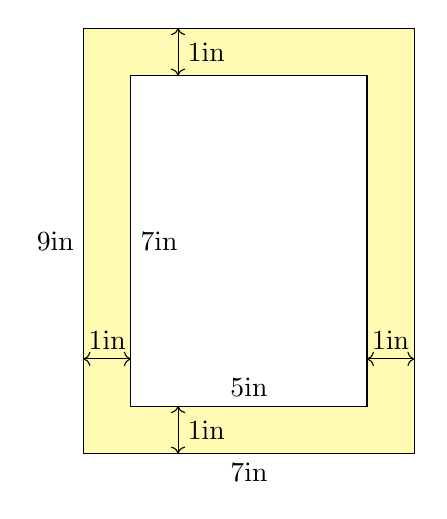
\begin{tikzpicture}[scale=0.6]
\draw[fill=yellow!30] (0,0) rectangle (7,9);
\draw[fill=white] (1,1) rectangle +(5,7);
\draw[<->] (0,2) -- (1,2) node [above,midway] {1in};
\draw[<->] (6,2) -- (7,2) node [above,midway] {1in};
\draw[<->] (2,0) -- (2,1) node [right,midway] {1in};
\draw[<->] (2,8) -- (2,9) node [right,midway] {1in};
\node at (1,4.5) [right] {7in};
\node at (3.5,1) [above] {5in};

\onslide<2->{\node at (0,4.5) [left] {9in};
\node at (3.5,0) [below] {7in};}
\end{tikzpicture}
\end{minipage}
\hspace{-1cm}
\begin{minipage}{0.35\textwidth}
\begin{align*}
\onslide<3->{\text{Area}_\text{frame} &= (9\times 7) - (5\times 7)} \\[10pt]
\onslide<4->{&= 63 - 35} \\[10pt]
\onslide<5->{&= 28\text{ in}^2}
\end{align*}
\end{minipage}
\end{frame}

\begin{frame}{Example 2}
What is the perimeter of $\triangle EFG$ if $E(3, 6), \, F(3, -2), \, G(-3, -2)$? 	\newline\\
\begin{minipage}{0.7\textwidth}
\onslide<2->{
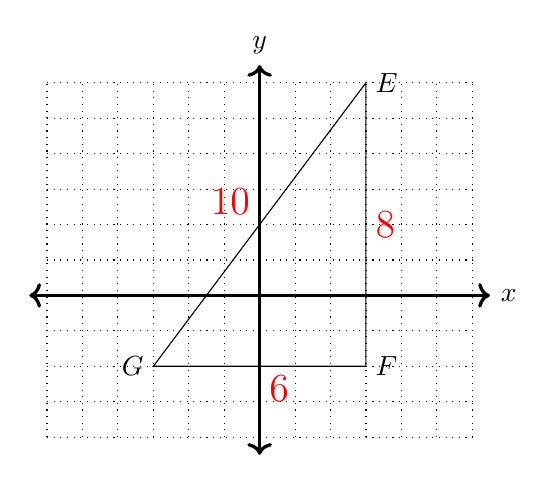
\begin{tikzpicture}[scale=0.45]
\coordinate (E) at (3,6);
\coordinate (F) at (3,-2);
\coordinate (G) at (-3,-2);
\draw[dotted] (-6,-4) grid (6,6);
\draw (E) node [right] {$E$} -- (F) node [right] {$F$} -- (G) node [left] {$G$} -- cycle;
\draw[very thick, <->] (-6.5,0) -- (6.5,0) node [right] {$x$};
\draw[very thick, <->] (0,-4.5) -- (0,6.5) node [above] {$y$};
\onslide<3->{
	\node at (0,-2) [below right, color=red] {\Large 6};
	\node at (3,2) [right,color=red] {\Large 8};
}
\onslide<4->{\node at (0,2) [above left, color=red] {\Large 10};}
\end{tikzpicture}}
\end{minipage}
\hspace{-0.5cm}
\begin{minipage}{0.2\textwidth}
\begin{align*}
\onslide<5->{\text{Perim.} &= 6+8+10} \\[8pt]
\onslide<6->{&= 24 \text{ units}}
\end{align*}
\end{minipage}
\end{frame}

\begin{frame}{Example 3}
Find the perimeter and area of each. Round your answers to 2 decimal places when necessary.	\newline\\	
(a)	\newline\\
\begin{minipage}{0.7\textwidth}
\begin{tikzpicture}[scale = 0.7]
    \tkzDefPoints{0/0/A, 6/0/B, 6/2/C, 4/2/D, 4/4/E, 2/4/F, 2/6/G, 0/6/H}
    \tkzDrawPolygon(A,B,C,D,E,F,G,H)
    \tkzMarkSegments[mark = ||](A,H A,B)
    \tkzMarkSegments[mark = |](B,C C,D D,E E,F F,G G,H)
    \tkzLabelSegment[left,xshift=-0.1cm](H,A){9 cm}
    \tkzLabelSegment[above,yshift=0.1cm](H,G){3 cm}
    \tkzMarkRightAngles(A,B,C B,C,D C,D,E D,E,F E,F,G F,G,H G,H,A B,A,H)
\end{tikzpicture}
\end{minipage}
\hspace{-0.5cm}
\begin{minipage}{0.25\textwidth}
\onslide<2->{Perim} \\ 
\onslide<3->{4(9) = 36 units}
\end{minipage}
\end{frame}

\begin{frame}{Example 3a}
\begin{minipage}{0.7\textwidth}
\begin{tikzpicture}[scale = 0.7]
    \tkzDefPoints{0/0/A, 6/0/B, 6/2/C, 4/2/D, 4/4/E, 2/4/F, 2/6/G, 0/6/H}
    \tkzDrawPolygon(A,B,C,D,E,F,G,H)
    \tkzMarkSegments[mark = ||](A,H A,B)
    \tkzMarkSegments[mark = |](B,C C,D D,E E,F F,G G,H)
    \tkzLabelSegment[left,xshift=-0.1cm](H,A){9 cm}
    \tkzLabelSegment[above,yshift=0.1cm](H,G){3 cm}
    \tkzMarkRightAngles(A,B,C B,C,D C,D,E D,E,F E,F,G F,G,H G,H,A B,A,H)
    \onslide<2->{\tkzDrawSegment[dashed,color=red](F,(2,0))
    \tkzDrawSegment[dashed,color=red](D,(4,0))}
    \onslide<3->{\node at (1,3) [color=red] {I};
    \node at (3,2) [color=red] {II};
    \node at (5,1) [color=red] {III};}
\end{tikzpicture}
\end{minipage}
\hspace{-0.5cm}
\begin{minipage}{0.25\textwidth}
\begin{align*}
\onslide<4->{\text{I}: 3(9) &= 27}	\\[8pt]
\onslide<5->{\text{II}: 3(6) &= 18}	\\[8pt]
\onslide<6->{\text{III}: 3(3) &= 9}	\\[8pt]
\end{align*}
\end{minipage}
\\[15pt]
\onslide<7->{Total Area: 27 + 18 + 9 = 54 sq. units}
\end{frame}

\begin{frame}{Example 3}
(b)	\newline\\
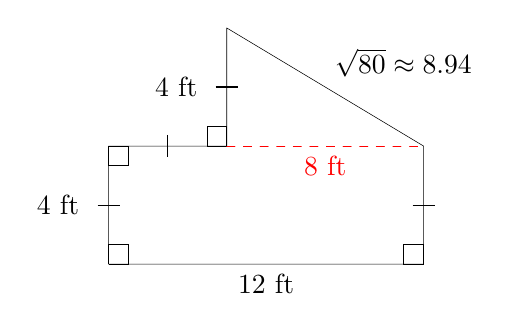
\begin{tikzpicture}
    \tkzDefPoints{0/1.5/F, 0/0/A, 4/0/B, 4/1.5/C, 1.5/1.5/E, 1.5/3/D}
    \tkzDrawPolygon(A,B,C,D,E,F)
    \tkzLabelSegment[below](A,B){12 ft}
    \tkzLabelSegment[left,xshift=-0.25cm](F,A){4 ft}
    \tkzMarkSegments[mark = |](A,F F,E E,D B,C)
    \tkzMarkRightAngles(B,A,F C,B,A E,F,A D,E,F)
    \onslide<2->{\tkzDrawSegment[dashed,color=red](E,C)}
    \onslide<3->{\tkzLabelSegment[below,color=red](E,C){8 ft}}
    \onslide<4->{\tkzLabelSegment[left,xshift=-0.25cm](D,E){4 ft}}
    \onslide<5->{\tkzLabelSegment[above right](C,D){$\sqrt{80} \approx 8.94$}}
\end{tikzpicture}
\newline\\
\onslide<6->{Perimeter:}
\onslide<7->{\[4+12+4+8.94+4+4\]} \\[-24pt]
\onslide<8->{\[36.94\text{ ft}\]}
\end{frame}

\begin{frame}{Example 2b}
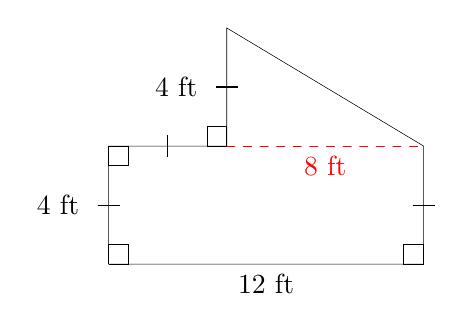
\begin{tikzpicture}
    \tkzDefPoints{0/1.5/F, 0/0/A, 4/0/B, 4/1.5/C, 1.5/1.5/E, 1.5/3/D}
    \tkzDrawPolygon(A,B,C,D,E,F)
    \tkzLabelSegment[below](A,B){12 ft}
    \tkzLabelSegment[left,xshift=-0.25cm](F,A){4 ft}
    \tkzMarkSegments[mark = |](A,F F,E E,D B,C)
    \tkzMarkRightAngles(B,A,F C,B,A E,F,A D,E,F)
    \tkzDrawSegment[dashed,color=red](E,C)
    \tkzLabelSegment[below,color=red](E,C){8 ft}
    \tkzLabelSegment[left,xshift=-0.25cm](D,E){4 ft}
\end{tikzpicture}
\newline\\
\onslide<2->{Triangle Area: $\frac{1}{2}(8)(4) = 16\text{ ft}^2$}	\newline\\
\onslide<3->{Rectangle Area: $4(12) = 48\text{ ft}^2$}	\newline\\
\onslide<4->{Total Area: 16 + 48 = 64 ft\textsuperscript{2}}
\end{frame}

\end{document}